\section{Privacy Preserving Histograms}\label{s:histograms}
Despite the challenges presented in sections \ref{s:challenges} and \ref{s:simple-algorithms}, the majority of algorithms can be transformed to their privacy preserving equivalent.
However, this is not a straightforward translation , as we examined in section \ref{s:simple-algorithms}, and in most cases it adds a complexity overhead to every algorithm that depends its control flow decisions in private data.

Histograms is a practical and notable example of algorithms that are widely used and the complexity of their privacy preserving version remains in computationally feasible levels, comparing to the textbook algorithm.
But first of all, what is a histogram?

As stated in \cite{ioannidis2003history}, histograms initially conceived as a visual aid to statistical approximations.
Webster’s defines a histogram as ``a bar graph of a frequency distribution in which the widths of the bars are proportional to the classes into which the variable has been divided and the heights of the bars are proportional to the class frequencies".
A histogram is generally a form of classifying and representing data in some categories of a specific range; the range is an individual ``base" element associated with each column.

More specifically, a histogram on some attributes $\{A, B, \dots, Z\}$ is constructed by partitioning the data distribution of those attributes into some ranges which are mutually disjoint subsets called buckets and approximating the frequencies and values in each bucket.
For the sake of simplicity let us suppose that the number of ranges ($\beta$) of all attributes are equal ($\beta \geq 1$).

In figure \ref{f:simple-hist} we present two histograms, the first one-dimensional over the attribute ``Patient Age" and the second is a two-dimensional over the attributes ``Patient Age" and ``Heart rate".
In both histograms $\beta = 4$, since the range of values for each attribute has been partitioned in four mutually disjoint subsets.
In the 1-dimensional histogram \ref{f:simple-hist}.a the $y-axis$ corresponds to the total number of occurrences of values that belong to each bucket.
In the 2-dimensional histogram \ref{f:simple-hist}.b since $y-axis$ corresponds to the ranges for the buckets for the second attribute, the occurrences are depicted with different colors.


\begin{figure}[h!]
    \centering
    \subfloat[1D Histogram]{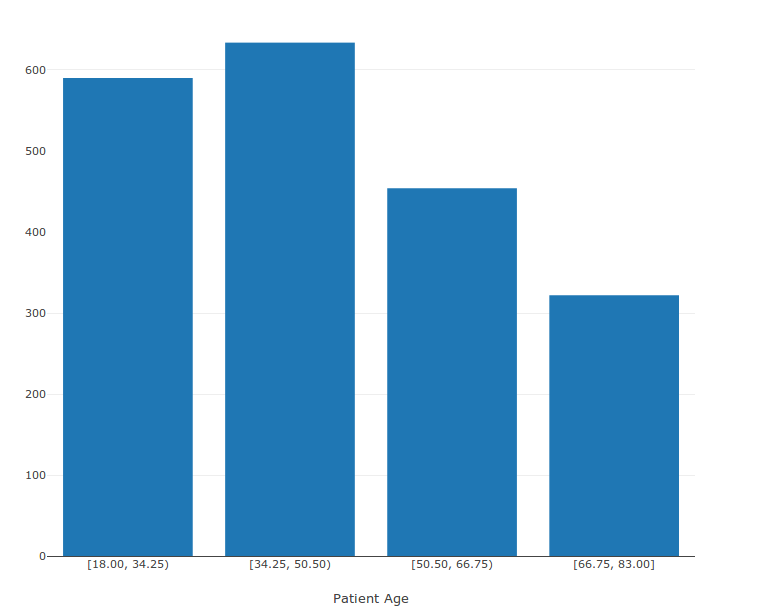
\includegraphics[width=0.49\columnwidth]{figures/1d-simple-hist.png}}
    \subfloat[2D Histogram / Heatmap]{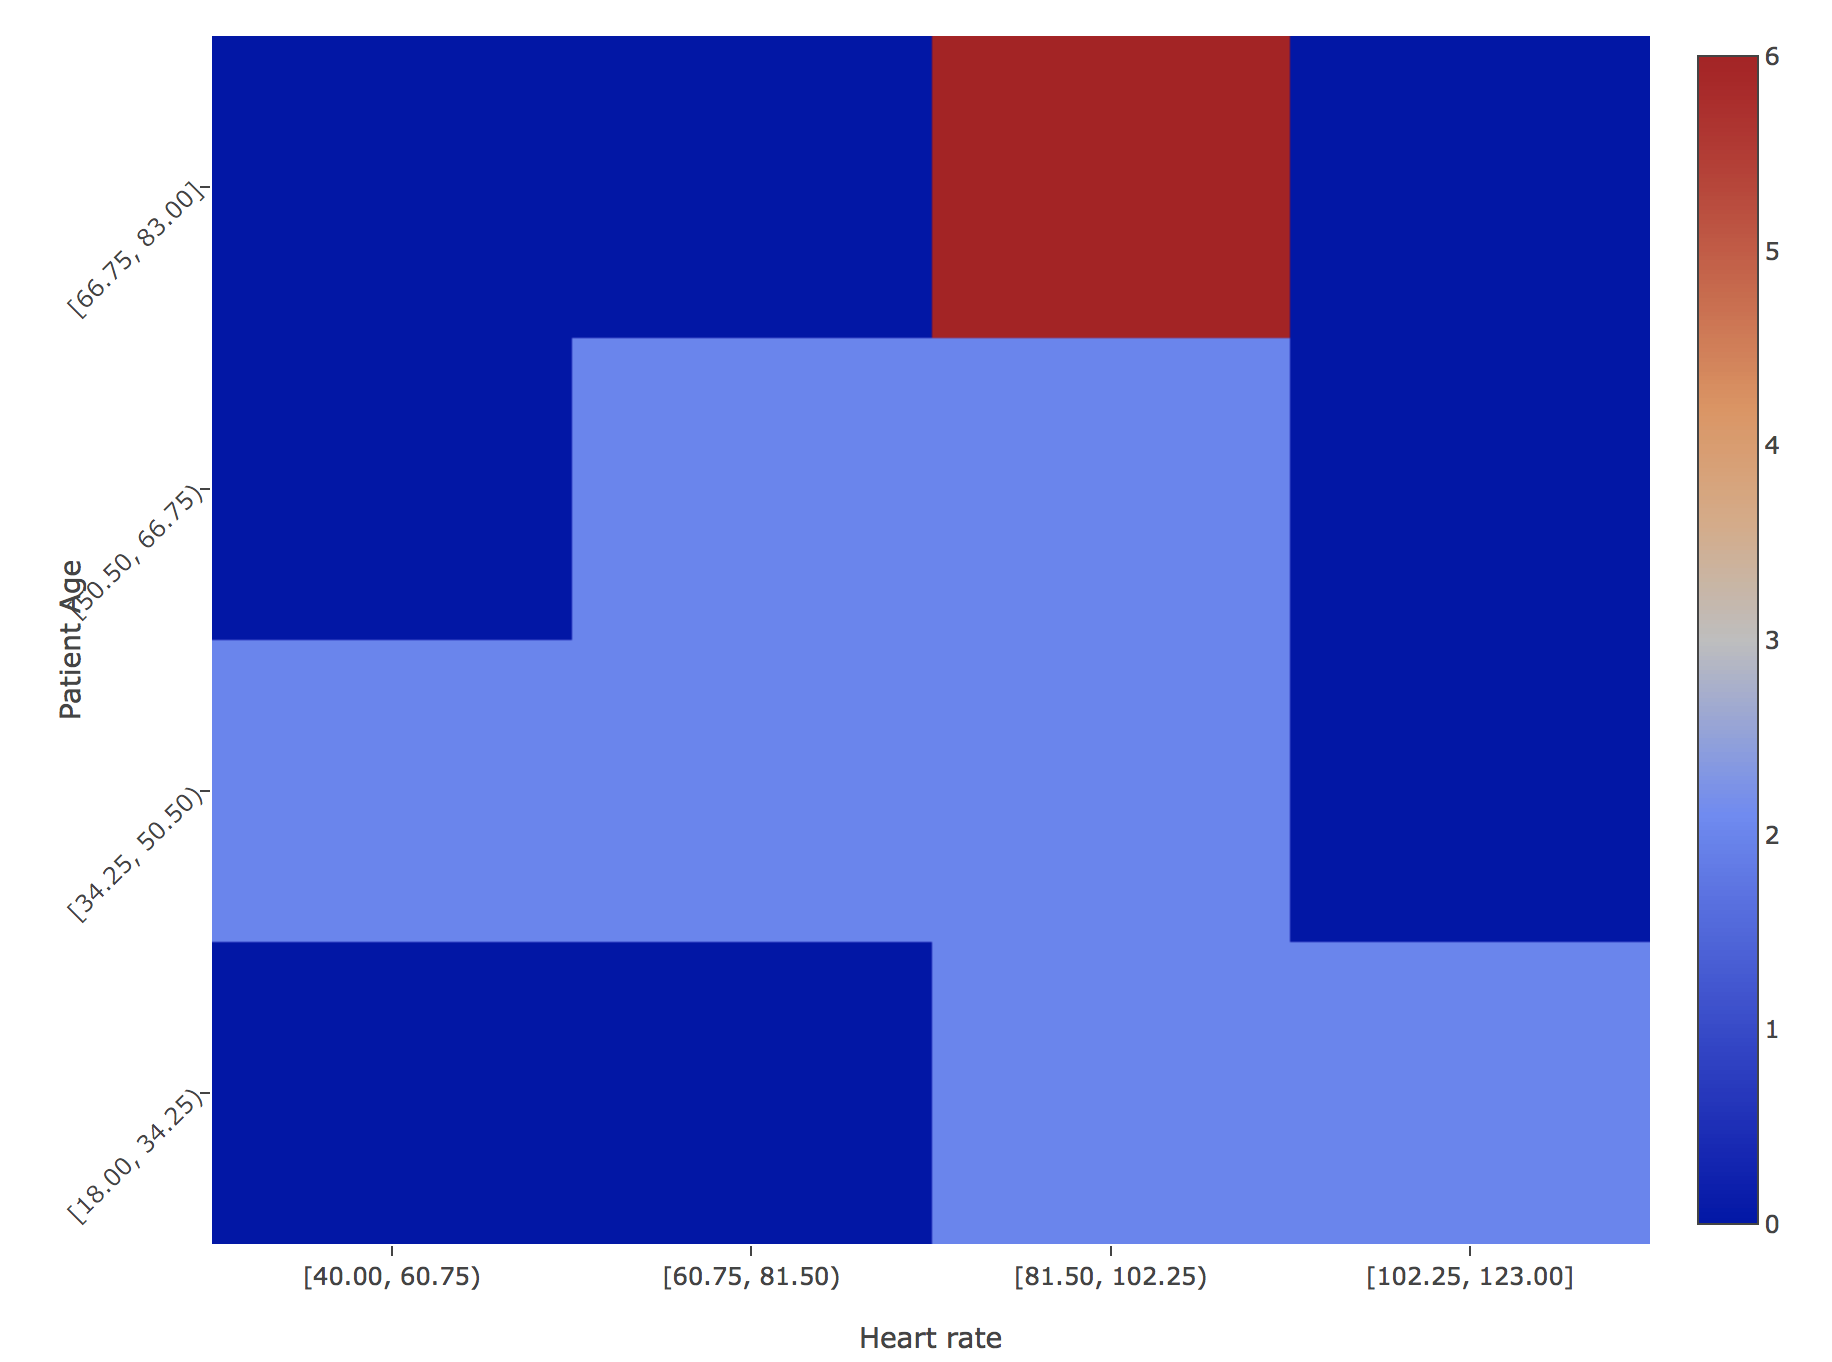
\includegraphics[width=0.49\columnwidth]{figures/2d-simple-hist.png}}

    \caption{(a) An one-dimensional histogram with $\beta = 4$
    (b) A two-dimensional histogram with $\beta = 4$.}
    \label{f:simple-hist}
\end{figure}


\fixme{in which cases is a histogram useful?}



\subsection{Agorithms for Privacy Preserving Histograms}\label{s:histogram-algos}

In algorithm \ref{a:1d-histogram-categorical} we present the privacy preserving algorithm of an one-dimensional (1D) histogram over categorical values.

\import{./}{algorithms/1d_hist_categorical.tex}

\fixme{explain the algorithm}



In algorithm \ref{a:1d-histogram-numerical} we present the privacy preserving algorithm of an one-dimensional (1D) histogram over numerical values.

\import{./}{algorithms/1d_hist_numerical.tex}

\fixme{explain the algorithm}



\import{./}{algorithms/multdim_hist_categorical.tex}

\fixme{explain the algorithm}



\import{./}{algorithms/multdim_hist_numerical.tex}

The algorithm computing a private multi-dimensional histogram is similar to the one regarding one-dimensional histograms but also addresses the issue of having a histogram of arbitrarily many dimensions.
In case we had a known number of dimensions the simplest solution would be to use nested loops, as many as the histogram dimensions.
Since the number of dimensions is not known, we have to think of something else.
We represent the multi-dimensional histogram as a serialized version with an one-dimensional array (a vector) instead of using a multi-dimensional array (a matrix).
For example a 2-dimensional $3 \times 4$ histogram will be represented as a vector whose length is $ 12 $ ($= 3 \cdot 4$), and a $3 \times 4 \times 5$ 3-dimensional histogram wit a vector of length $ 60 $ ($= 3 \cdot 4 \cdot 5$)

When it comes to indexing if we wish to access the 2-dimensional $N \times M$ histogram represented as an one-dimensional at row $ i $ and column $ j $, instead of using $h[i][j]$ we use $h[i \cdot M + j]$.
Similarly, for the 3-dimensional $L \times N \times M$ histogram, $h[i][j][k]$ becomes $h[i \cdot N \cdot M + j \cdot M + k]$. So there needs to be a computation of a single index based on the multiple dimension indexes. In algorithm \ref{a:multidim-histogram-numerical}, the \texttt{positions} vector holds this index for each record of the provided array, as can bee seen in lines $ 12 $ and $ 13 $



